\chapter{\label{cha:sts_transformers}Adapting Transformers for STS}

Transformers can be considered as the biggest revolution happened in NLP, in recent years. Like Recurrent Neural Networks (RNNs), transformers are designed to handle sequential input data, such as natural language, for tasks like machine translation and text summarisation. However, unlike RNNs, transformers do not necessarily process the data in order. Rather, the attention mechanism in transformers provides context for any position in the input sequence. For example, if the input data is a sentence, the transformer does not need to process the beginning of the sentence before the end. Since RNNs process the data in order, they often forget the content of distant positions in the sequence and cause problems when processing longer sequences. Furthermore, since RNNs process word by word, it is hard to parallelise the work for processing sentences. The attention mechanism in transformers can address both of these issues \autocite{10.5555/3295222.3295349}.


Transformers were first introduced in \autocite{10.5555/3295222.3295349}, where they use a transformer architecture for sequence to sequence tasks like machine translation. The authors show that an architecture with only attention-mechanisms without any RNNs can improve on the results in sequence to sequence tasks. The first notable research in using transformers for language modelling was OpenAI GPT \autocite{radford2018improving}. OpenAI GPT adopts a pre-training followed by fine-tuning scheme which means that once pre-trained, it can be fine-tuned to a large number of down-stream NLP tasks like text classification, named entity recognition etc. However, the first breakthrough in using transformer models for language modelling happened with the introduction of BERT \autocite{devlin-etal-2019-bert}. As we explain in Section \ref{sec:transformers_related}, BERT employs a masked language modelling (MLM) objective which brings improvements over OpenAI GPT. Later, different variants to BERT were proposed by the community. We explain some of these models that we used in this chapter in Section \ref{sec:transformers_related}. All of these transformer models, follow the same fine-tuning scheme of OpenAI GPT.


Transformer models, which we have considered in this chapter use special tokens to obtain a single contiguous sequence for each input sequence. Specifically, the first token is always a special classification token \textsc{[CLS]} and sentence pairs are separated using a special token \textsc{[SEP]}. The final hidden state of \textsc{[CLS]}  is used for sentence-level fine-tuning tasks and the final hidden state of each token is used for token-level fine-tuning tasks. The fine-tuning scheme in transformers is usually simple like adding a softmax layer on top of \textsc{[CLS]} token for the text classification tasks. Furthermore, the fine-tuning scheme is very efficient as the parameters in the transformer model are already optimised with the pre-training process. Therefore, transformer models have been extremely popular and successful in many NLP tasks \autocite{devlin-etal-2019-bert}. 

In this chapter, we explore different transformers models in variety of STS experiments. 
We address four research questions in this chapter:

\textbf{RQ1:} How well the existing state-of-the-art transformer models perform in STS task? 

\textbf{RQ2:} Can the method further improved with transfer learning and data augmentation techniques?

\textbf{RQ3:} Can the transformer model be easily adopted in to different languages?

\textbf{RQ4:} How well the proposed transformer models perform in a different domain? 

The main contributions of this chapter are as follows.

\begin{enumerate}
\item We evaluate five popular transformer models in three English STS datasets. We compare the results with the previous methods and show that transformer based STS methods outperform all the other STS methods we have experimented.

\item We propose further enhancements to the architecture using inter dataset transfer learning and data augmentation.  

\item We evaluate how well the transformer models perform on STS datasets in different languages and domains. 

\item The code and the pre-trained models are publicly available to the community\footnote{The public GitHub repository is available on \url{https://github.com/tharindudr/STS-Transformers}}. We have published the code as a python library \footnote{The developed python library is available on \url{https://pypi.org/project/ststransformers/}} and by the time of writing this chapter, it has more than 3,000 downloads from the community. 

\end{enumerate}

The rest of this chapter is organised as follows. Section \ref{sec:transformers_related} describes the pre-trained transformer models we used in this chapter. Section \ref{sec:transformer_method} discusses the architecture and \ref{sec:transformer_english} describes the experiments done with three English STS datasets. Section \ref{sec:transformer_transfer} and \ref{sec:transformer_aug} provide more experiments to improve the results. Experiments done with other languages and domains are shown in Section \ref{sec:transformer_multilingual} and Section \ref{sec:transformer_domain}. Section \ref{sec:transformer_siamese} discusses recent developments done with transformers and Siamese architectures, addressing a key issue in using transformers in STS. The chapter finishes with conclusions and ideas for future research directions in transformers. 

\section{Related Work}
\label{sec:transformers_related}
As we mentioned before, after the introduction of BERT \autocite{devlin-etal-2019-bert}, many variants of different transformer models have been proposed by adding minor modifications to the original BERT transformer. Usually these modifications has resulted in improvements in the fine-tuning scheme for the down-stream NLP tasks. Expecting a similar behaviour for the STS task too, we considered following transformer models for the experiments in this chapter.

\paragraph{BERT} \autocite{devlin-etal-2019-bert} proposes a MLM objective, where some of the tokens of a input sequence are randomly masked, and the objective is to predict these masked positions taking the corrupted sequence as input. BERT applies a Transformer encoder to attend to bi-directional contexts during pre-training. In addition, BERT uses a next-sentence-prediction (NSP) objective. Given two input sentences, NSP predicts whether the second sentence is the actual next sentence of the first sentence. The NSP objective aims to improve the tasks, such as question answering and natural language inference, which require reasoning over sentence pairs. 

\paragraph{RoBERTa} \autocite{liu2019roberta} makes a few changes to the BERT architecture and achieves substantial improvements. The changes include: (1) Training the model longer with larger batches and more data; (2) Removing the NSP objective; (3) Training on longer sequences; (4) Dynamically changing the masked positions during pre-training.

\paragraph{ALBERT} \autocite{Lan2020ALBERT} proposes two parameter-reduction techniques (factorised embedding parameterisation and cross-layer parameter sharing) to lower memory consumption and speed up training. Furthermore, ALBERT \autocite{Lan2020ALBERT} argues that the NSP objective in BERT lacks difficulty, as the negative examples are created by pairing segments from different documents, this mixes topic prediction and coherence prediction into a single task. ALBERT instead uses a sentence-order prediction
(SOP) objective. SOP obtains positive examples by taking out two consecutive segments and negative examples by reversing the order of two consecutive segments from the same document.


\paragraph{ELECTRA} Compared to BERT, ELECTRA \autocite{Clark2020ELECTRA} proposes a more effective pre-training method. Instead of corrupting some positions of inputs with [MASK], ELECTRA replaces some tokens of the inputs with their plausible alternatives sampled from a small generator network. ELECTRA trains a discriminator to predict whether each token in the corrupted input was replaced by the generator or not. The pre-trained discriminator can then be used in downstream tasks for fine-tuning, improving upon the pre-trained representation learned by the generator.

\paragraph{XLNET} \autocite{yang2019xlnet} identifies a key weakness in BERT pre-training. \autocite{yang2019xlnet} argues that the symbols such as \textsc{[MASK]} that are introduced by BERT during pre-training, causes discrepancy between pre-training and fine-tuning as they never occur in real data. Therefore, XLNET suggests a new auto-regressive method based on permutation language modelling (PLM) \autocite{JMLR:v17:16-272} without introducing any new symbols. 

Upon the introduction, all of these transformer models have been evaluated in many down-stream NLP tasks including STS too. However, there is no comprehensive study done on STS using transformers considering big and small datasets, transfer learning, data augmentation, multilingual STS etc. which we do in this chapter.

\section{Transformer Architecture for STS}
\label{sec:transformer_method}

The transformer architecture for STS is shown in Figure \ref{fig:sts_transformers}. The input of this model is a concatenation of the two sentences, separated by the \textsc{[SEP]} token. Then the output of the \textsc{[CLS]} token is used as the input of a softmax layer that predicts the similarity of the two sentences. We used mean-squared-error loss as the objective function. As the configurations, we used a batch-size of eight, Adam optimiser with learning rate $2\mathrm{e}{-5}$, and a linear learning rate warm-up over 10\% of the training data. During the training process, the parameters of the transformer, as well as the parameters of the subsequent layers, were updated. The models were trained using only training data. Furthermore, they were evaluated while training after each 100 batches, using an evaluation set that had one fifth of the rows in training data. We performed early stopping if the evaluation loss did not improve over ten evaluation steps. All the models were trained for three epochs. As these transformer models are computationally expensive, we used an Nvidia Tesla T4 GPU for the training process. We have kept these configuration same for all the experiments; in order to ensure consistency between all the languages and domains. This also provides a good starting configuration for researchers who intend to use transformers on a new language pair. The implementation is based on PyTorch \autocite{NEURIPS2019_9015} and HuggingFace \autocite{wolf-etal-2020-transformers}.

\begin{figure}[ht]
	\centering
	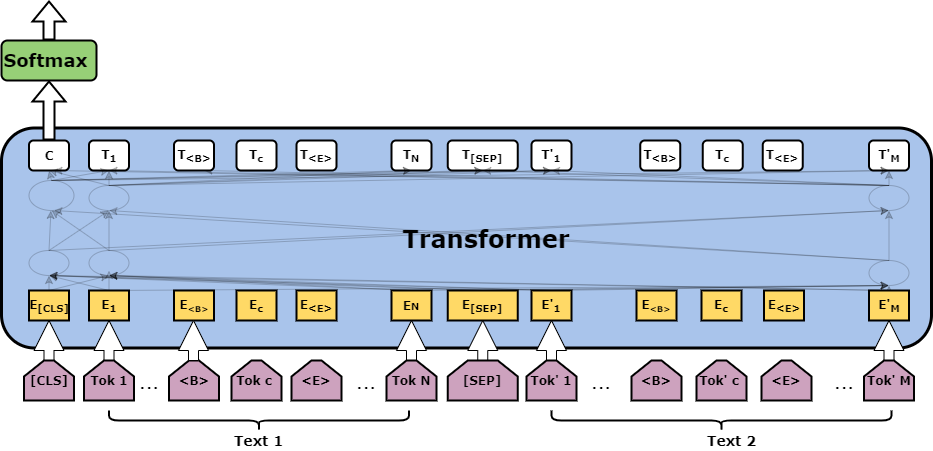
\includegraphics[scale=0.4]{figures/semantic_textual_similarity/transformers/STSTransformers.png}
	\caption[Architecture for using Transformers in STS]{Architecture for using Transformers in STS.}
	\label{fig:sts_transformers}
\end{figure}

\section{Exploring Transformers in English STS}
\label{sec:transformer_english}
We evaluated all the above transformer variations in the three English STS datasets we introduced in \ref{cha:sts_introduction}; SICK, STS 2017 and QUORA. All of the transformer models we considered have several models that supports English (e.g.\ \textit{bert-large-cased} \& \textit{bert-base-cased} for BERT, \textit{albert-xxlarge-v2} \& \textit{albert-base-v2} for ALBERT) and usually the large models outperform the smaller models in downstream tasks. Therefore, we used the largest possible model that our GPU setup can load with each transformer type; \textit{bert-large-cased} for BERT \autocite{devlin-etal-2019-bert}, \textit{albert-large-v2} for ALBERT \autocite{Lan2020ALBERT}, \textit{roberta-large} for RoBERTa \autocite{liu2019roberta}, \textit{google/electra-large-discriminator} for ELECTRA \autocite{Clark2020ELECTRA} and \textit{xlnet-large-cased}  \autocite{yang2019xlnet} for XLNET. All of these models are available in HuggingFace \autocite{wolf-etal-2020-transformers} model hub\footnote{Models are available on \url{https://huggingface.co/models}}.

We trained the transformer models on the training sets on those datasets and evaluated them on the testing sets. The results are shown in Table \ref{tab:sick_transformers}, Table \ref{tab:sts_transformers} and Table \ref{tab:quora_transformers} respectively. 

\begin{table*}[htb]
	%\footnotesize
	\centering
	\scalebox{0.95}{
		\begin{tabular}{|l|cc|}
			\hline
			\textbf{Model} & $\bm{\rho}$   & $\bm{\tau}$     
			\\ \hline
			\textit{BERT}                  
			& 0.881 & 0.826  \\
			\textit{ALBERT}                  
			& 0.886 & 0.829  \\
			\textit{RoBERTa}                  
			& 0.892$^{\dagger}$ & 0.834$^{\dagger}$  \\
			\textit{ELECTRA}                  
			& 0.872 & 0.819  \\
			\textit{XLNET}                  
			& 0.879 & 0.821  \\
			\hline
		\end{tabular}
	}
	\caption[Results for SICK with Transformer Models]{Results for SICK dataset with different variants of transformer models. For each variant, Pearson Correlation ($\bm{\rho}$) and Spearman Correlation ($\bm{\tau}$) are reported between the predicted values and the gold labels of the test set. Best result from all the variations is marked with ${\dagger}$.}  
	\label{tab:sick_transformers}
\end{table*}


\begin{table*}[htb]
	%\footnotesize
	\centering
	\scalebox{0.95}{
		\begin{tabular}{|l|cc|}
			\hline
			\textbf{Model} & $\bm{\rho}$   & $\bm{\tau}$     
			\\ \hline
				\textit{BERT}                  
		& 0.889 & 0.858  \\
		\textit{ALBERT}                  
		& 0.874 & 0.852  \\
		\textit{RoBERTa}                  
		& 0.895$^{\dagger}$ & 0.861$^{\dagger}$  \\
		\textit{ELECTRA}                  
		& 0.873 & 0.849  \\
		\textit{XLNET}                  
		& 0.868 & 0.843  \\
			\hline
		\end{tabular}
	}
	\caption[Results for STS 2017 with Transformers]{Results for STS 2017 dataset with different variants of Transformers. For each variant, Pearson Correlation ($\bm{\rho}$) and Spearman Correlation ($\bm{\tau}$) are reported between the predicted values and the gold labels of the test set. Best result from all the variations is marked with ${\dagger}$. }  
	\label{tab:sts_transformers}
\end{table*}


\begin{table*}[htb]
	%\footnotesize
	\centering
	\scalebox{0.95}{
		\begin{tabular}{|l|c|}
			\hline
			\textbf{Model} & RMSE     
			\\ \hline
			\textit{BERT}                  
			& 0.349   \\
			\textit{ALBERT}                  
			& 0.354   \\
			\textit{RoBERTa}                  
			& 0.359   \\
			\textit{ELECTRA}                  
			& 0.353   \\
			\textit{XLNET}                  
			& 0.346$^{\dagger}$   \\
			\hline
		\end{tabular}
	}
	\caption[Results for QUORA with Transformers]{Results for QUORA dataset with different variants of Transformers. For each variant, Root Mean Squared Error (RMSE) reported between the predicted values and the gold labels of the test set. Best result from all the variations is marked with ${\dagger}$. }  
	\label{tab:quora_transformers}
\end{table*}

As can be seen in Table \ref{tab:sick_transformers} and \ref{tab:sts_transformers}, for SICK and STS 2017 datasets, RoBERTa outperformed other transformer models. Since SICK and STS 2017 are smaller datasets, optimised nature in RoBERTa seems to be beneficial in smaller datasets. In the QUORA dataset, which is considerably bigger than SICK and STS 2017, \textit{XLNET}  outperforms other transformer models. However, from the results, there is no clear indication that which transformer model would perform best in a certain dataset other than the fact that 	\textit{RoBERTa} performs slightly better in smaller datasets. It should be noted that, all of the transformers perform on par with each other. 

In the initial experiments, we noticed that the transformer models are quite sensitive to the random seed\footnote{Random seed is used to configure the starting weights in a neural network. Keeping the random seed constant from one experiment to the next removes the variation due to this randomness, making it easier to interpret the effects of other design changes such as hyper parameter values.} of the experiments \autocite{zhang2021revisiting}. Changing the random seed led to very different results. To minimise this affect from random seed, we conducted the experiments for five different random seeds and took the mean of these experiments as the final results which is the value reported in Tables \ref{tab:sick_transformers}, \ref{tab:sts_transformers} and \ref{tab:quora_transformers}. We noticed that doing many experiments with different random seeds reduced the variance of the final result. 

With this we answer our \textbf{RQ1}: transformers can be successful adopted in the STS task and they produce good results in all the datasets. For the smaller datasets, \textit{RoBERTa} performed slightly better than other transformer models. Furthermore, we recommend to conduct more experiments with different random seeds in order to minimise the variance.


\subsection{Impact of Transfer Learning}
\label{sec:transformer_transfer}
Similar to the \textit{Siamese neural networks} in Chapter \ref{cha:sts_siamese_neural_networks}, we explored the impact of transfer learning  in STS, with transformers too. We saved the weights of the transformers models that were trained on each STS dataset; SICK, STS 2017 and QUORA. We specifically used the two models that performed best in these dataset; RoberTa and XLNET. We again initiated training for each dataset, however rather than training the transformer model from scratch, we used the weights of the models trained on other STS dataset. We compared this transfer learning results to the results we got from training the model from scratch. Similar to the \textit{Siamese neural network} experiments, we conducted this transfer learning experiment only on STS2017 and SICK dataset since the QUORA dataset was already big and transfer learning from a smaller dataset to a larger dataset won't make much sense.


\begin{table*}[htb]
	%\footnotesize
	\centering
	\scalebox{0.95}{
		\begin{tabular}{|l|c|c|}
			\hline
			\textbf{Start Model} & STS2017 & SICK      
			\\ \hline
			\textit{STS2017$_{RoBERTa}$}                  
			& 0.895 & \textcolor{gray}{(+0.009)} \\
			\textit{STS2017$_{XLNET}$}                     
			& 0.868 & \textcolor{gray}{(+0.011)}  \\
			\hline
			\textit{SICK$_{RoBERTa}$}                     
			& \textcolor{gray}{(+0.008)} & 0.892 \\
			\textit{SICK$_{XLNET}$}                     
			& \textcolor{gray}{(+0.013)} & 0.879 \\
			\hline
			\textit{QUORA$_{RoBERTa}$}                     
			& \textcolor{gray}{(-0.025)}  &  \textcolor{gray}{(-0.021)}    \\
			\textit{QUORA$_{XLNET}$}                     
			& \textcolor{gray}{(-0.039)} &  \textcolor{gray}{(-0.043)}    \\
			\hline
		\end{tabular}
	}
	\caption[Results for transfer learning with Transformers]{Results for transfer learning with different Transformers. For each transfer learning experiment we show the difference between with transfer learning and without transfer learning. Non-grey values are the results of the experiments without transfer learning which we showed in the previous section too. We only report the Pearson correlation due to ease of visualisation.}  
	\label{tab:transfer_transformers}
\end{table*}

As can be seen in Table \ref{tab:transfer_transformers}, when we performed transfer learning from STS2017 $\Rightarrow$ SICK and SICK $\Rightarrow$ STS2017 the results improve. This shows that transfer learning can improve the results in transformers. However, similar to the \textit{Siamese neural networks}, when we performed transfer learning from QUORA $\Rightarrow$ STS2017 and QUORA $\Rightarrow$ SICK the results did not improve, in fact, they decrease. Therefore, we can assume that  performing transfer learning from a very different dataset, is not beneficial in transformers too. 

We can conclude that transfer learning can improve the results for transformers too in STS. However, the transfer learning dataset should be picked carefully considering the similarity of the two datasets too, rather than only considering the size of the dataset.

\subsection{Impact of Data Augmentation}
\label{sec:transformer_aug}
Since the transformer models have provided better results with more training data, we experimented the impact of data augmentation with the transformer models. Similar to \textit{Siamese neural networks} in Chapter \ref{cha:sts_siamese_neural_networks}, we employed thesaurus-based augmentation in which 10,000 additional training examples are generated by replacing random words with one of their synonyms found in Wordnet \autocite{10.1145/219717.219748}. We specifically used the two models that performed best with the bigger dataset and smaller dataset; \textit{RoBERTa} and \textit{XLNET}. Since the transfer learning improved the results in previous experiment, we trained the augmented training set on the transferred models; models trained on STS2017 for SICK experiments and models trained on SICK for STS2017. The results are shown in Table \ref{tab:augmentation_transformers}. 

\begin{table*}[htb]
	%\footnotesize
	\centering
	\scalebox{0.95}{
		\begin{tabular}{|c|c|c|}
			\hline
			\textbf{Dataset} &	\textbf{Start Model} &  $\bm{\rho}$      
			\\ \hline
			\multirow{ 2}{*}{\textit{SICK}}	& \textit{STS2017$_{RoBERTa}$}                  
			& \textcolor{gray}{(+0.012)} \\
			&	\textit{STS2017$_{XLNET}$}                     
			& \textcolor{gray}{(+0.011)}  \\
			\hline
			\multirow{ 2}{*}{\textit{STS2017}}  & \textit{SICK$_{RoBERTa}$}                     
			& \textcolor{gray}{(+0.014)}  \\
			& \textit{SICK$_{XLNET}$}                     
			& \textcolor{gray}{(+0.013)} \\
			\hline
		\end{tabular}
	}
	\caption[Results for data augmentation with Transformers]{Results for data augmentation with different Transformers. For each data augmentation experiment we show the difference between with dat augmentation and without data augmentation. We only report the Pearson correlation ($\bm{\rho}$) due to ease of visualisation.}  
	\label{tab:augmentation_transformers}
\end{table*}

As can be seen in the results, data augmentation improved the results of all the experiments with transformers. However, even with the additional 10,000 training instances, \textit{RoBERTa} outperformed \textit{XLNET}. We can conclude that simple data augmentation techniques can improves the performance of transformers too in STS task. From the experiments we conducted, our best result for both STS2017 and SICK datasets were provided by \textit{RoBERTa} when combined with both transfer learning and data augmentation.


This answers our \textit{RQ2} in this Chapter, we can use transfer learning and simple data augmentation techniques to improve the results of transformers too in STS. 

\begin{table*}[htb]
	%\footnotesize
	\centering
	\scalebox{0.95}{
		\begin{tabular}{|l|c|}
			\hline
			\textbf{Model} & $\bm{\rho}$      
			\\ \hline
			\cite{jimenez-etal-2014-unal} & 0.807 \\
			\cite{bjerva-etal-2014-meaning} & 0.827 \\
			\cite{zhao-etal-2014-ecnu-one} & 0.841 \\
			\textit{Siamese GRU} & 0.882  \\
			\textit{RoBERTa} & 0.920  \\
			\hline
		\end{tabular}
	}
	\caption[Results comparison for SICK with leader board results including transformers]{Results for SICK dataset with different transformer models. For each variant, Pearson Correlation ($\bm{\rho}$) is reported between the predicted values and the gold labels of the test set.}  
	\label{tab:sick_transformers_all}
\end{table*}

\begin{table*}[htb]
	%\footnotesize
	\centering
	\scalebox{0.95}{
		\begin{tabular}{|l|c|}
			\hline
			\textbf{Model} & $\bm{\rho}$      
			\\ \hline
			\cite{tian-etal-2017-ecnu} & 0.851 \\
			\cite{maharjan-etal-2017-dt} & 0.854 \\
			\cite{cer-etal-2017-semeval}  & 0.855   \\
			\textit{Siamese GRU} & 0.862  \\
			\textit{RoBERTa} & 0.915  \\
			\hline
		\end{tabular}
	}
	\caption[Results comparison for STS2017 with leader board results]{Results for STS2017 dataset with different variants of Siamese Neural Network. For each variant, Pearson Correlation ($\bm{\rho}$) is reported between the predicted values and the gold labels of the test set.  }  
	\label{tab:sts_transformers_all}
\end{table*}

Furthermore, we compared the results of the best transformer model with the best results submitted to the competitions \autocite{cer-etal-2017-semeval, marelli-etal-2014-semeval} and with the supervised and unsupervised STS methods we have experimented so far in this part of the thesis. As can be seen in Table \ref{tab:sick_transformers_all} and \ref{tab:sts_transformers_all} \textit{RoBERTa} outperforms the best system submitted to both competition. It also outperforms the unsupervised and supervised STS methods we have so far explored in this part of the thesis including \textit{Siamese neural networks} too. Therefore, we can conclude that transformers are the current state-of-the-art for English STS.

\section{Portability to Other Languages}
\label{sec:transformer_multilingual}
Similar to the other STS methods we have experimented in this part of the thesis, we evaluated transformers in Arabic STS and Spanish STS datasets that were introduced in Chapter \ref{cha:sts_introduction}. Transformers too has the advantage that it does not rely on language dependent features.  As a result, the approach is easily portable to other languages given the availability of pre-trained transformer models in that particular language. As pre-trained transformer models, we used AraBERT and AraELECTRA for Arabic which were trained on Arabic Wikipedia dump, the 1.5B words Arabic Corpus \autocite{elkhair201615}, the OSCAR corpus \autocite{ortiz-suarez-etal-2020-monolingual} and the OSIAN Corpus \autocite{zeroual-etal-2019-osian} using original BERT and ELECTRA architectures we explained in Section \ref{sec:transformers_related}\footnote{More details about the models and download links are available on \url{https://github.com/aub-mind/arabert}}. Both of the models use Farasa segmentation as a pre-processing step \autocite{abdelali-etal-2016-farasa}. For Spanish, we used BETO; Spanish BERT model \autocite{CaneteCFP2020} which was trained on Spanish Unannotated Corpora\footnote{Corpora is available on \url{https://github.com/josecannete/spanish-corpora}} using original BERT architecture\footnote{More details about BETO is available on \url{https://github.com/dccuchile/beto}}. Additionally for both languages, we used the "BERT-Base, Multilingual Cased" model \autocite{devlin-etal-2019-bert} which has been built on the top 100 languages with the largest Wikipedias that includes Arabic and Spanish languages too.

The results are shown in Table \ref{tab:arabic_transformers_all} for Arabic and Table \ref{tab:spanish_transformers_all}. We also compared the results of the transformer models with the best results submitted to the competition \autocite{cer-etal-2017-semeval} and with the supervised/unsupervised STS methods we have experimented so far in this part of the thesis. 


\begin{table*}[htb]
	%\footnotesize
	\centering
	\scalebox{0.95}{
		\begin{tabular}{|l|c|}
			\hline
			\textbf{Model} & $\bm{\rho}$      
			\\ \hline
			\cite{tian-etal-2017-ecnu} & 0.744 \\
			\cite{nagoudi-etal-2017-lim} & 0.746 \\
			\cite{wu-etal-2017-bit}  & 0.754   \\
			\textit{Siamese GRU} & 0.763  \\
			\textit{mBERT} & 0.778\\
			\textit{AraElectra} & 0.791\\
			\textit{AraBERT} & 0.794 \\
			\hline
		\end{tabular}
	}
	\caption[Results comparison for Arabic STS with leader board results]{Results for Arabic STS dataset with different transformers. For each variant, Pearson Correlation ($\bm{\rho}$) is reported between the predicted values and the gold labels of the test set.  }  
	\label{tab:arabic_transformers_all}
\end{table*}


\begin{table*}[htb]
	%\footnotesize
	\centering
	\scalebox{0.95}{
		\begin{tabular}{|l|c|}
			\hline
			\textbf{Model} & $\bm{\rho}$   \\  
			\hline
			\cite{hassan-etal-2017-fcicu} & 0.848 \\
			\cite{wu-etal-2017-bit} &  0.850 \\
			\cite{tian-etal-2017-ecnu} & 0.855 \\
			\textit{Siamese GRU} & 0.863  \\
			\textit{mBERT} & 0.884  \\
			\textit{BETO} & 0.890  \\
			\hline
		\end{tabular}
	}
	\caption[Results comparison for Spanish STS with leader board results]{Results for Spanish STS dataset with different variants of Siamese Neural Network. For each variant, Pearson Correlation ($\bm{\rho}$) is reported between the predicted values and the gold labels of the test set. }  
	\label{tab:spanish_transformers_all}
\end{table*}

As can be seen in the results transformer based STS method outperformed all the other supervised and unsupervised STS models in both languages and outperforms the top systems of the competition in both languages. From the experimented pre-trained transformer models, language specific models like BETO, AraBERT outperformed general multilingual models.  Therefore, we can conclude that  transformers are currently the state-of-the-art for Arabic and Spanish STS too. Furthermore, it should be noted that it is very easy to adopt transformers in a different language. We only changed the pre-trained model to the new language and performed the training. 

This answers our \textbf{RQ3:}, the transformers can be successfully adopted in different languages by changing the pre-trained model and the training dataset and it provides state-of-the-art results in STS.

\section{Potability to Other Domains}
\label{sec:transformer_domain}
In order to answer our \textit{RQ4}; how well the proposed transformer models can be applied in STS tasks in different domains, we evaluated our method on Bio-medical STS dataset explained in \ref{cha:sts_introduction} (BIOSSES). As we mentioned before Bio-medical STS dataset does not have a training set. Therefore, we had to follow a transfer learning strategy to evaluate it on the Bio-medical STS dataset. Similar to \textit{Siamese neural network} experiments in Chapter \ref{cha:sts_siamese_neural_networks}, we used the pre-trained English STS transformer models and performed inference on the Bio-medical STS dataset. 

For this transfer learning strategy we considered two pre-trained transformer models; \textit{bert-large-cased} \autocite{devlin-etal-2019-bert} (We refer this as \textit{BERT}) which we used in previous experiments too and BioBERT \autocite{10.1093/bioinformatics/btz682} which has trained BERT on PubMed abstracts\footnote{More details and the model are available on \url{https://github.com/dmis-lab/biobert}}.

\begin{table*}[htb]
	%\footnotesize
	\centering
	\scalebox{0.95}{
		\begin{tabular}{|l|c|c|}
			\hline
			\textbf{Data} & \textbf{BERT} & \textbf{BioBERT}      
			\\ \hline
			\textit{STS2017}                  
			& 0.663 & 0.763 \\
			\textit{SICK}                     
			& 0.658 & 0.751  \\
			\textit{QUORA}                     
			& 0.612 & 0.682 \\
			\hline
		\end{tabular}
	}
	\caption[Results for transfer learning with transformers in BIOSSES dataset]{Results for transfer learning with transformers in BIOSSES dataset. Two considered pre-trained transformer models are textbf{BERT} and \textbf{BioBERT}. We only report the Pearson correlation due to ease of visualisation.}  
	\label{tab:transfer_transformers_biosses}
\end{table*}


As can be seen in the Table \ref{tab:transfer_transformers_biosses}, transformers provided satisfactory results in Bio-medical STS. We got the best result from transformers when trained on STS 2017 using BioBERT. Furthermore, there was a clear improvement when the English STS model was trained using BioBERT rather than using general BERT. This can be due to the fact that most of the Bio-medical words that appear in BIOSSES dataset are out of vocabulary in general BERT model which can cause problems to the neural network when it observes them in the testing phase. Furthermore, it should be noted that in this experiment too, when we performed transfer learning from QUORA dataset the results are lower than performing transfer learning from SICK or STS 2017. This again can be due to the reason SICK and STS 2017 datasets have a similar annotation strategy to the BIOSSES dataset as we discussed in Chapter \ref{cha:sts_introduction}. These results are similar to what we saw with \textit{Siamese neural networks} in Chapter \ref{cha:sts_siamese_neural_networks}.

\begin{table*}[htb]
	%\footnotesize
	\centering
	\scalebox{0.90}{
		\begin{tabular}{|l|c|}
			\hline
			\textbf{Model} & $\bm{\rho}$   \\  
			\hline
			\textit{ELMo $\bigoplus$ BERT}  &  0.708 \\
			\textit{Siamese GRU$_{STS2017}$} & 0.719 \\
			\cite{10.1093/bioinformatics/btx238} & 0.754 \\
			\textit{BioBERT$_{STS2017}$} & 0.763 \\
			\textit{BioSentVec} \autocite{8904728} & 0.810  \\
			\hline
		\end{tabular}
	}
	\caption[Results comparison for BIOSSES with top results and transformers]{Results for BIOSSES dataset with transformers compared with top results reported for BIOSSES. For each variant, Pearson Correlation ($\bm{\rho}$) is reported between the predicted values and the gold labels of the test set. }  
	\label{tab:biosses_transformers_all}
\end{table*}

Furthermore we compared our results with the best results reported for the dataset. The results are shown in Table \ref{tab:biosses_transformers_all}. The best model we had in Table \ref{tab:transfer_transformers_biosses} which is based on BioBERT when trained on STS2017, is represented as \textit{BioBERT$_{STS2017}$}. As shown in the results, our method provides satisfactory results when compared with best approaches. Also, it outperforms the GRU based \textit{Siamese neural network} architecture we experimented in Chapter \ref{cha:sts_siamese_neural_networks} using the same transfer learning strategy. However, it should be noted that the unsupervised method we experimented in Chapter \ref{cha:sts_sentence_encoders} with BioSentVec \autocite{8904728} comfortably outperformed the transformer based STS method we experimented in this Chapter.

With these observations, we can answer our \textbf{RQ4: How well the proposed transformer models perform in a different domain?}. The transformers can be adopted to STS in different domains just by only changing the pre-trained transformer model. However, without a proper training set the results won't be strong. This is a common observation we had for supervised STS methods in this chapter.

\section{Recent Developments: Siamese Transformers}
\label{sec:transformer_siamese}

\begin{figure}[ht]
	\centering
	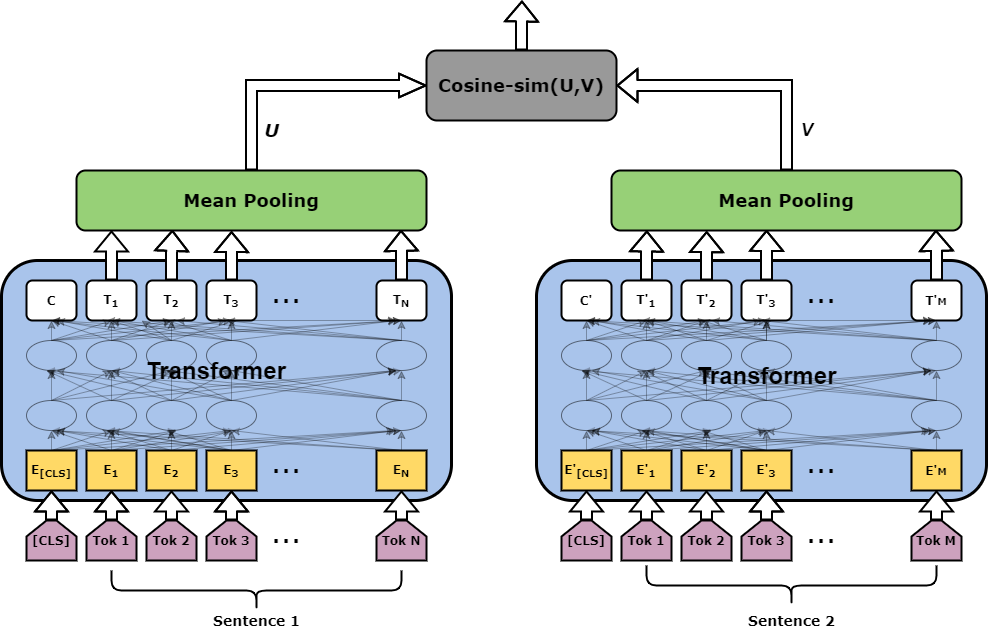
\includegraphics[scale=0.35]{figures/semantic_textual_similarity/transformers/sentence-bert.png}
	\caption[Architecture for using Siamese Transformers in STS]{Architecture for using Siamese Transformers in STS.}
	\label{fig:siamese_transformers}
\end{figure}

As we observed in previous experiments, transformers are state-of-the-art in supervised STS. However, to predict the similarity in test time, both of the sentences are required to be fed into the network. Two sentences are passed to the transformer network
and the similarity is predicted. However, this setup is unsuitable for various text similarity tasks due to too many possible combinations. Finding in a collection of n = 10 000 sentences the pair with the highest similarity requires $n \times \frac {(n-1)}{2} = 49,995,000$ inference computations with the default transformer architecture we experimented in this chapter. On a modern V100 GPU, this requires about 65 hours. Similarly, finding which of the over 40 million existent questions of Quora is the most similar for a new question could be modelled as a pair-wise comparison with the same architecture, however, answering a single query would require over 50 hours. This massive computational overload would not be suitable for many real-world applications \autocite{reimers-gurevych-2019-sentence}.

The obvious solution to this would be to get sentence embeddings from the transformer network. A common approach would be to use vector aggregation methods that we already used in Chapter \ref{cha:sts_state_of_the_art_methods}. However, we previously showed that these simple, unsupervised vector aggregation methods get outperformed by sentence encoders that used traditional word embeddings. Therefore, \autocite{reimers-gurevych-2019-sentence} propose a Siamese neural architecture based on transformers. The architecture is shown in Figure \ref{fig:siamese_transformers}, which is very similar to the Siamese architectures we experimented in Chapter \ref{cha:sts_siamese_neural_networks}.

This architecture can be trained on a STS dataset. As this is a Siamese architecture, it can produce sentence embeddings that can be used at the inference time without having both sentences in the network. \autocite{reimers-gurevych-2019-sentence} show that this architecture provides less accuracy than the default transformer architecture in STS tasks, yet the results are very compatible and outperform other sentence encoders like Universal Sentence Encoder and Infersent. Furthermore, it outperforms the word embedding based Siamese neural network architectures we experimented in Chapter \ref{cha:sts_siamese_neural_networks}. Therefore, this architecture is the current state-of-the-art Siamese neural network in STS tasks. \autocite{reimers-gurevych-2019-sentence} calculate that complexity for finding the most similar sentence pair in a collection of 10,000 sentences is reduced from 65 hours with the default architecture to the computation of 10,000 sentence embeddings (~5 seconds with Siamese transformer architecture) and computing cosine similarity (~0.01 seconds). We can conclude that this architecture would be very efficient in many NLP applications where it is required to find similar sentences from a large set of sentences, such as Translation Memories\footnote{More details and the pre-trained models on Siamese transformers are available on \url{https://www.sbert.net/}}. 


\section{Conclusions}
In this chapter, we experimented with utilising state-of-the-art transformers in STS task. We evaluated the default sentence pair regression architecture on transformers in three English datasets, two non-English datasets and a bio-medical STS dataset. For the smaller STS datasets; SICK and STS2017 we show that \textit{RoBERTa} outperforms other transformer models and for the larger STS dataset, \textit{XLNET} outperforms the baseline. Also, we show that we can improve the results more with transfer learning and data augmentation techniques. For the three English datasets and two non-English datasets transformer based STS method outperforms all the other supervised and unsupervised STS methods we have experimented with in this part of the thesis. Furthermore, they also outperform the best systems submitted to each shared task which shows that transformers are the current state-of-the-art in supervised STS.

However, in the BIOSSES dataset where it does not have a training set, we used a transfer learning based zero-shot learning when applying transformers. Even though transformers outperformed other STS methods we experimented like Siamese neural networks, they could not outperform the sentence vector based method we explored in Chapter \ref{cha:sts_sentence_encoders}. We can conclude that despite the fact that the transformers can be adopted in different domains by changing the word embedding model, they won't provide strong results without a proper training set. 

One major limitation in the transformer based STS method is that it requires to have both sentences in the network at the inference time which can cause a massive computational overhead for some NLP applications. To overcome this, \autocite{reimers-gurevych-2019-sentence} propose Siamese transformers architecture which is capable of proving sentence vectors. Another limitation is the big model size in transformer based methods. The pre-trained transformer models are quite big and can cause problems in real-world applications. As a solution to this, we hope to explore knowledge distillation \autocite{Gou2021} in STS task as future work. In knowledge distillation, transformer based methods can be used as teacher-models to train simple student-models like Siamese GRU, which in turn would be able to provide competitive results to transformer based methods. 

With this, we conclude Part I of the thesis. We explored numerous STS methods that are based on word vectors and easy to adopt in different languages and domains. We evaluated them on different STS datasets and discussed their benefits and limitations in each Chapter. We can conclude that transformers are state-of-the-art in supervised STS methods and sentence encoders are state-of-the-art in unsupervised STS methods. Keeping in mind the benefits and limitations of these STS methods, in the next two parts in the thesis, we are going to employ them in two applications in translation technology; translation memories in Part II and translation quality estimation in Part III.

